\chapter{La zone de visualisation}
\section{Pr�sentation}
La zone de visualisation est la zone la plus importante de
l'application. En effet, c'est sur cette zone que s'afficheront les
diff�rentes pages. Par exemple, lors de la visualisation d'un projet,
la version en HTML du projet appraitra dans la zone de visualisation.\\ 
Voici une description des pages apparaissant sur dans
cette zone.\newpage
\section{Mes enseignements}
Voici les diff�rentes �tapes lorsque l'enseignant clique sur {\it Mes
enseignements}.\\ Commen�ons par la sp�cification de la premi�re page apparaissant.
\subsection{Page principale}
\begin{flushleft}
\scalebox{0.6}{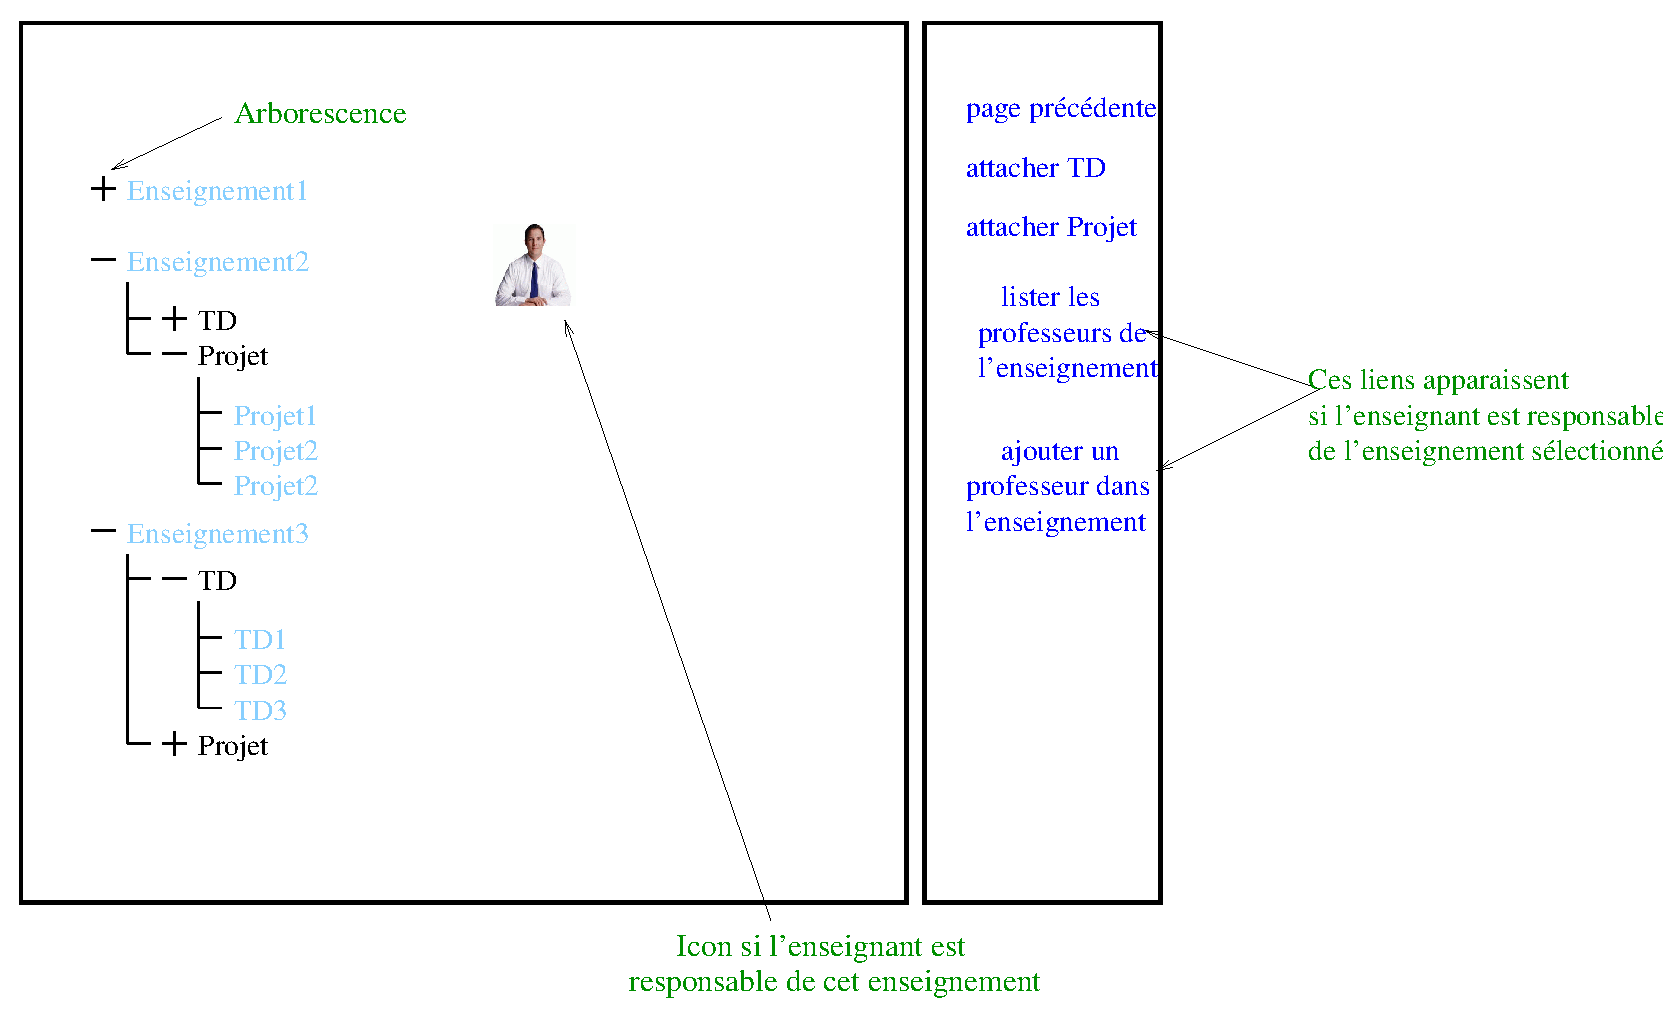
\includegraphics{../eps/MesEnseignements.eps}}\\
{\it Premi�re page de Mes enseignements}
\end{flushleft}
Cette page repr�sente un listing de tous les enseignements dans
lesquels l'enseignant connect� appratient. Si l'enseignant
est responsable d'un des enseignements, alors une icon apparait � c�t�
de l'enseignement.\\De plus, si l'enseignant selectionne un
enseignement dans lequel il est responsable, de nouveaux
fonctionnalit�s (liens) appraissent dans la zone annexe.
\newpage

Lors de la consultation de ses enseignements, l'enseignant peut
attacher un projet � un de ses enseignements.
\begin{flushleft}
\scalebox{0.5}{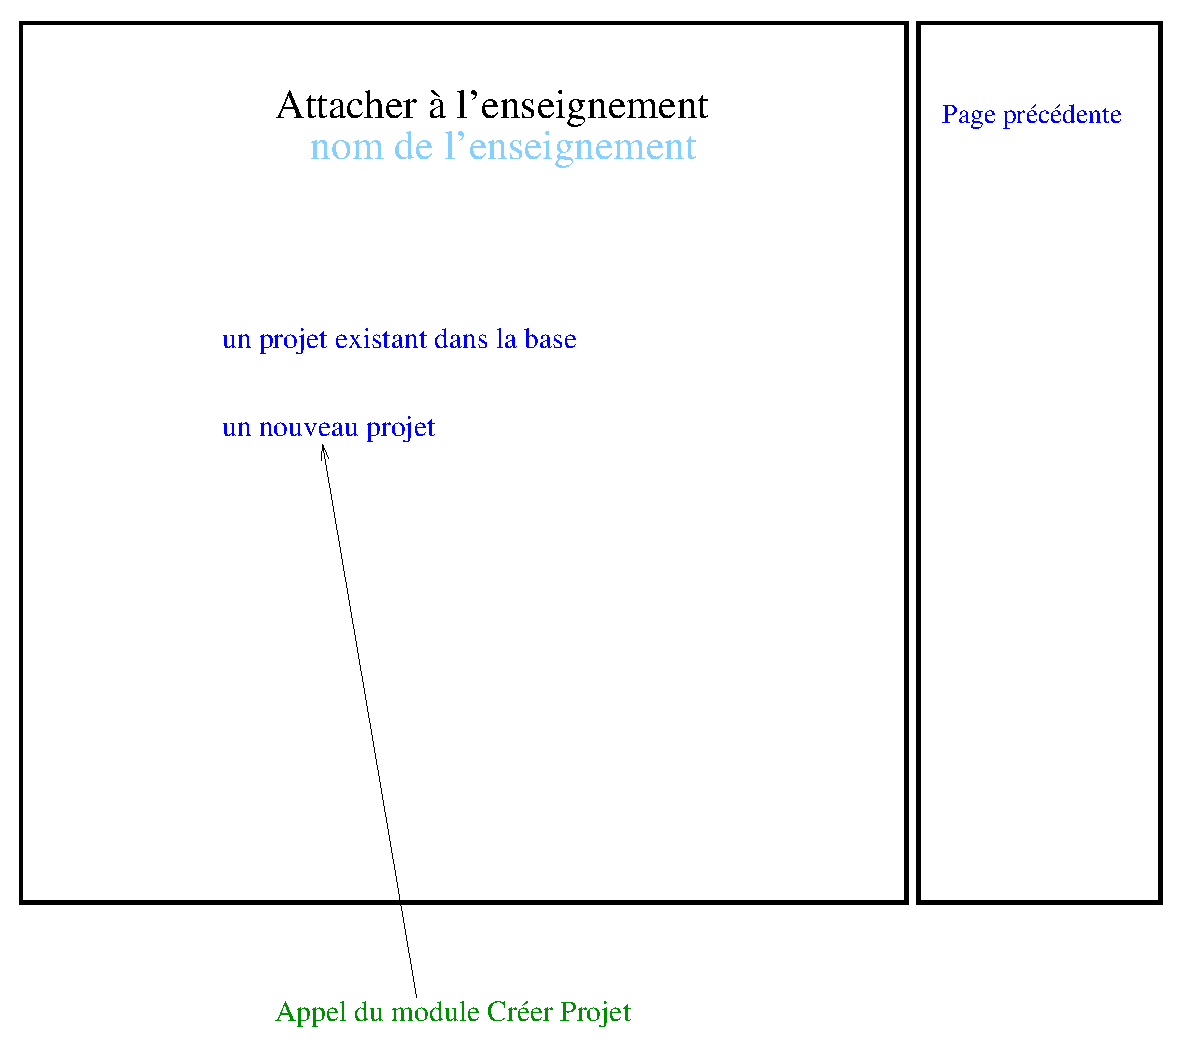
\includegraphics{../eps/Attacher1Projet.eps}}\\
{\it Page principale de l'attachement d'un projet}
\end{flushleft}
Lorsque que l'enseignant choisit d'attacher un projet pr�sent dans la
base de l'apllication, apparait une nouvelle fen�tre contenant la liste
des projets class�s par enseignements.
\begin{flushleft}
\scalebox{0.5}{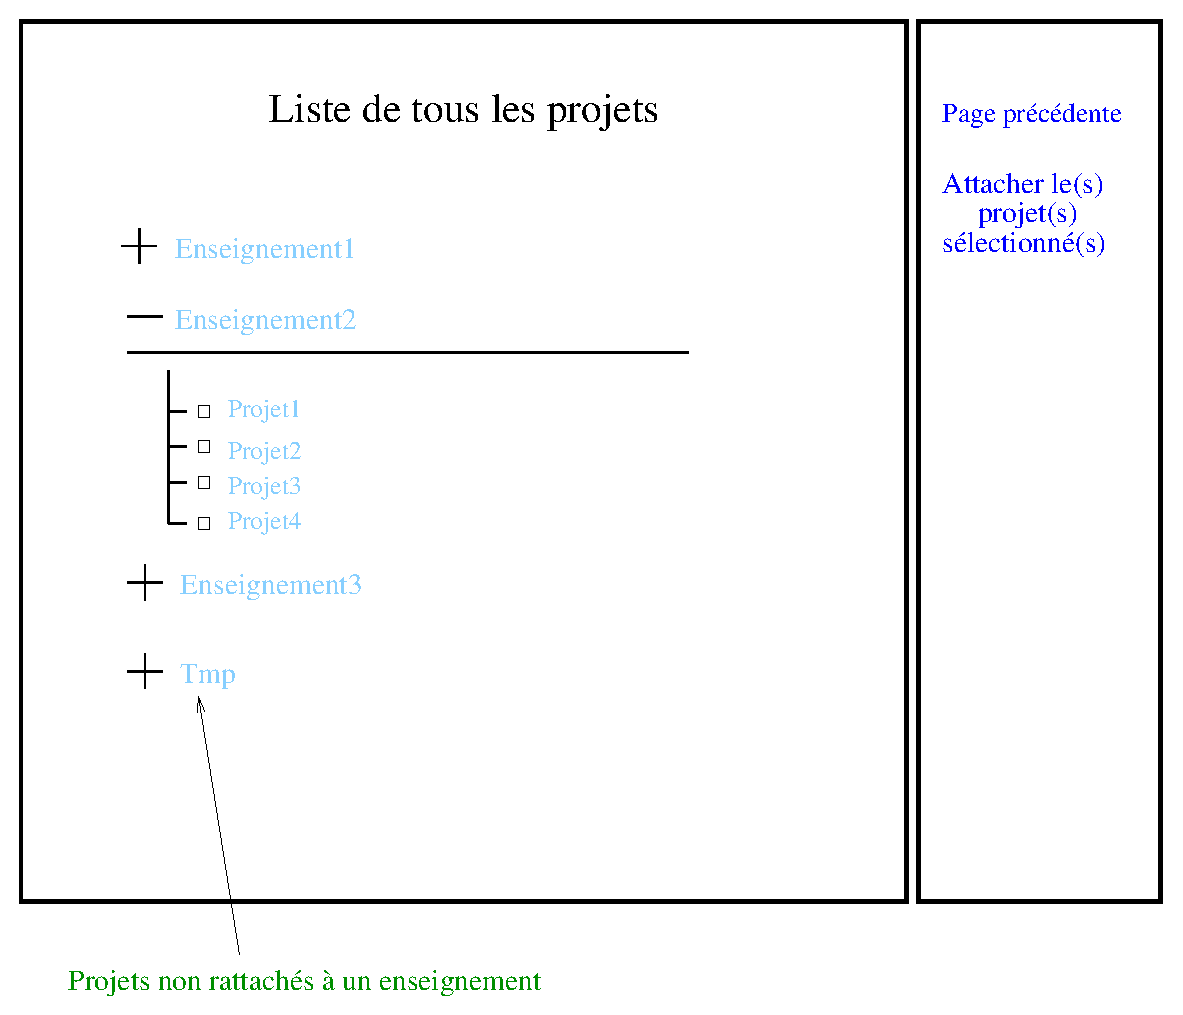
\includegraphics{../eps/AttacherProjetExistant.eps}}\\
{\it Liste des projets pouvant �tre attach�s}
\end{flushleft}
\newpage
\subsection{Attacher un TD}
Lors de la consultation de ses enseignements, l'enseignant peut
attacher un TD � un de ses enseignements.
\begin{flushleft}
\scalebox{0.5}{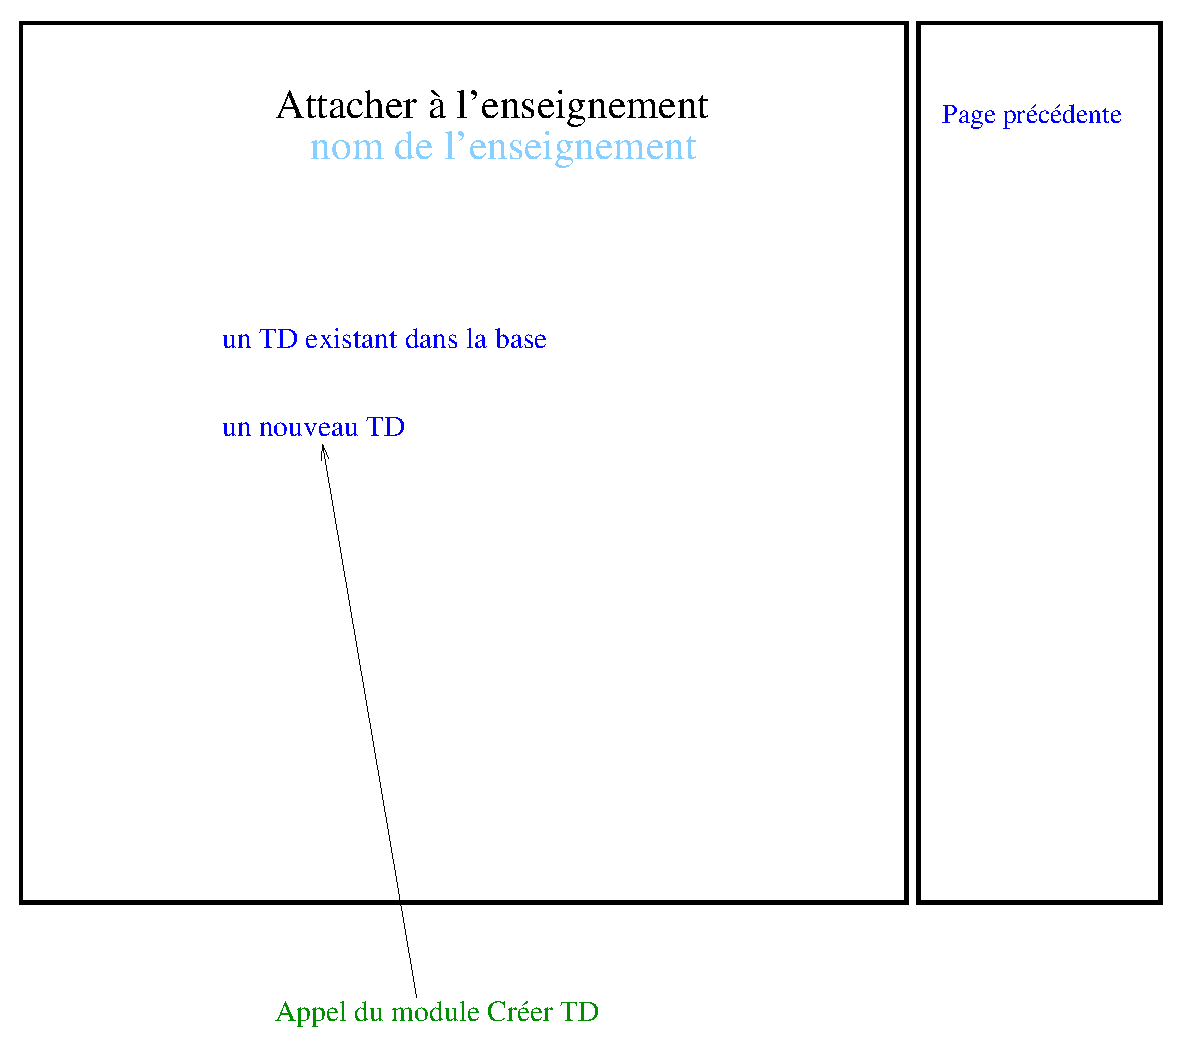
\includegraphics{../eps/Attacher1TD.eps}}\\
{\it Page principale de l'attachement d'un TD}
\end{flushleft}

Lorsque que l'enseignant choisit d'attacher un TD pr�sent dans la
base de l'apllication, apparait une nouvelle fen�tre contenant la liste
des TD class�s par enseignements.
\begin{flushleft}
\scalebox{0.5}{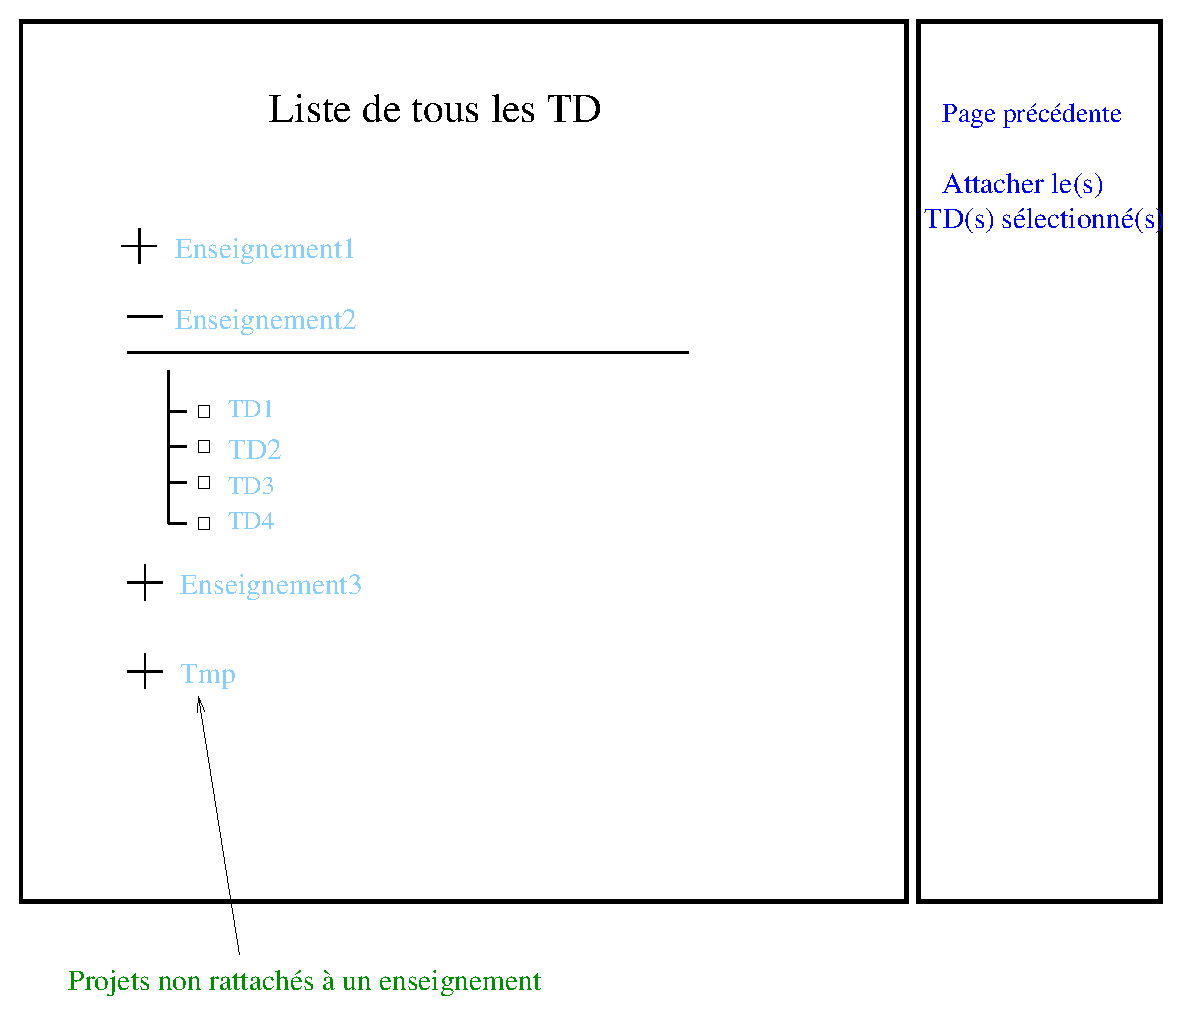
\includegraphics{../eps/AttacherTDExistant.eps}}\\
{\it Liste des TD pouvant �tre attach�s}
\end{flushleft}

\subsection{Liste des professeurs de l'enseignement}
Le responsable d'un enseignement � la possibilit� de lister tous les
enseignants de son enseignement. Ainsi, il peut g�rer les droits dans
son enseignement c'est-�-dire ajouter ou retirer les droits � des
enseignants pour acc�der � leur enseignement. 
\begin{flushleft}
\scalebox{0.5}{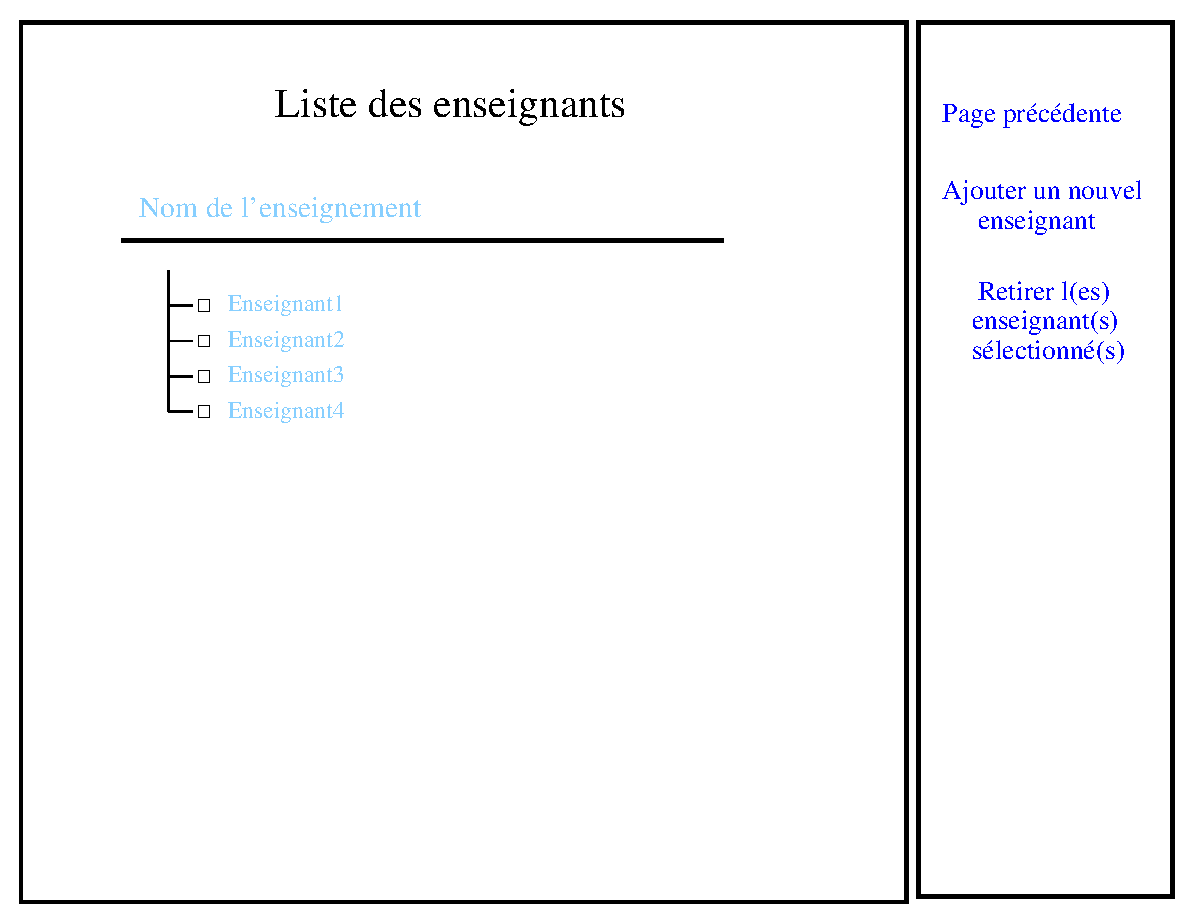
\includegraphics{../eps/ListingProfD1Enseignement.eps}}\\
{\it Liste des professeurs de l'enseignement}
\end{flushleft}

\begin{flushleft}
\scalebox{0.5}{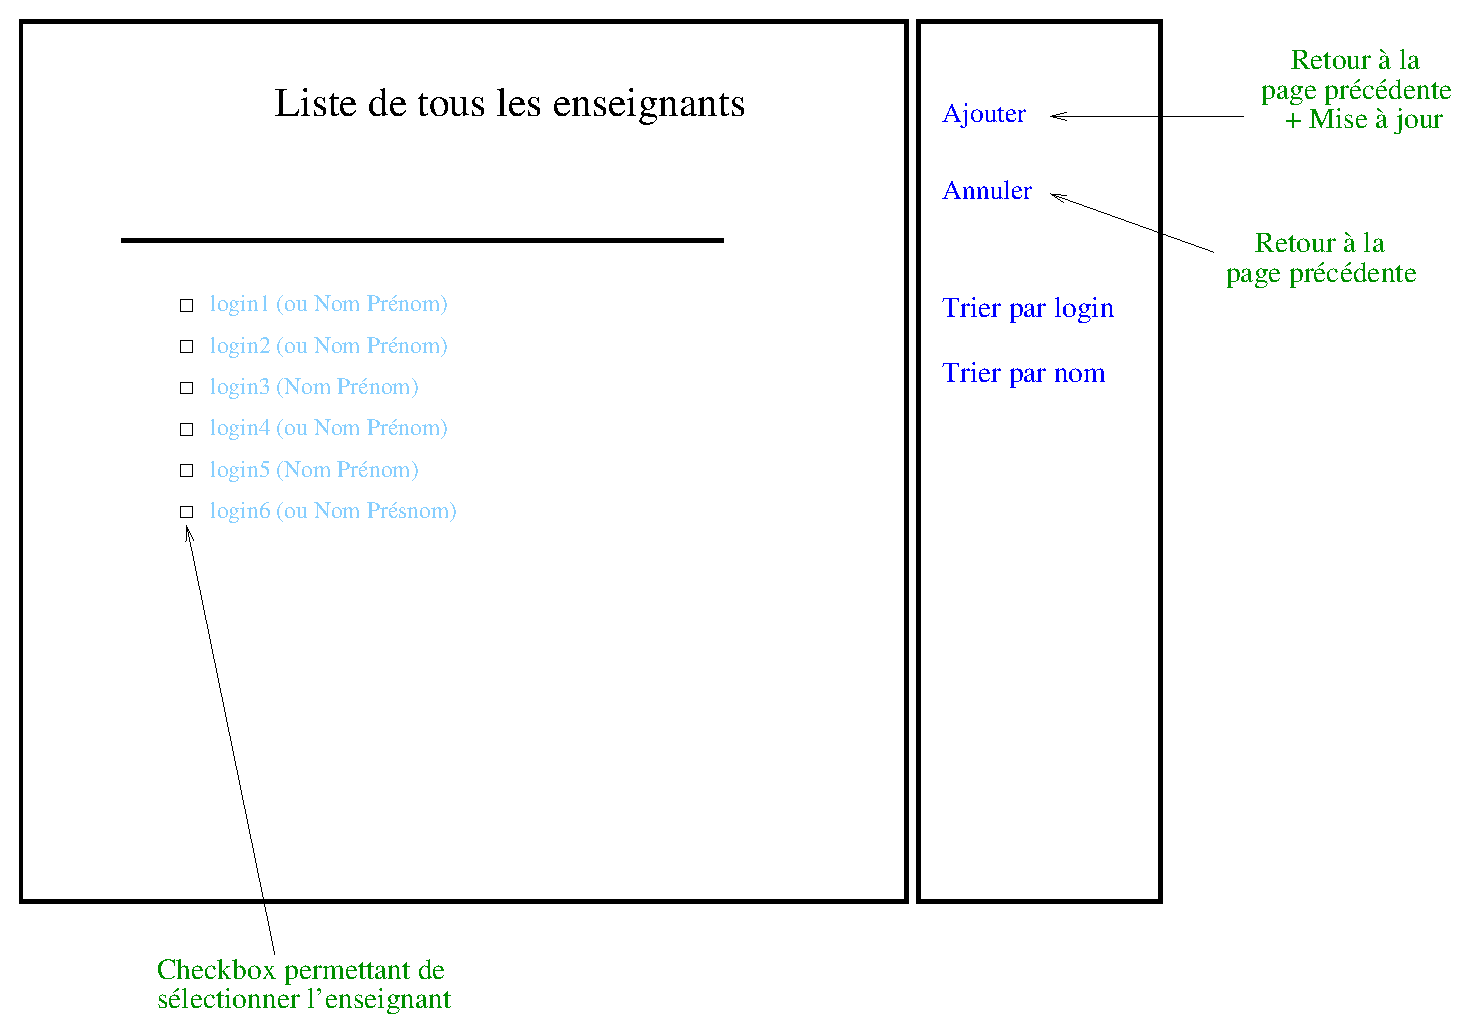
\includegraphics{../eps/AjoutD1NouveauProf.eps}}\\
{\it Liste de tous les professeurs de la base sauf ceux de l'enseignement}
\end{flushleft}





